\section{My favourite gadgets in 2050}
I have told before that my favourite gadgets are mobile and computer. Gradually both of the gadgets are being advanced time to time. In 2050, these devices will be updated more and more. I think by the welfare of nano-technology both are device will be so small and more powerful that we can not imagine. Using these devices in 2050 different types of tasks could be done in few seconds.
\subsection{Computer in 2050}
Computer is very important devices. We can solve any problem using the device. We are using computers and laptops for gaming and other purposes. A best configured computer is prerequisite for gaming and other purposes. In figure~\ref{fig:fig6}, I have shown a gaming computer.
\begin{figure}[h]
    \centering
    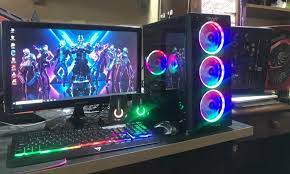
\includegraphics[width = 0.8\textwidth]{pic/gaming.jpeg}
    \caption{Gaming computer}
    \label{fig:fig6}
\end{figure}\\
 I expect that technology will bring something advanced in future for our laptops/computers. I think that in 2050 gaming computer will be so advanced such that we are playing video game in real life. I think that video game will be controlled by human fingers and faces and human sound. Such as when A gamer will say open computer then gaming computer will start. When he/she will say open game then a specific game will be started  and will be ready for gaming. And the actions of the game will be controlled by face and fingers. The characters of the game will be controlled by fingers and faces. Such as when A gamer will move his/her fingers left or right then the character of the game will move left or right respectively.\\
 In~\cite{c.realme.comWebsite},Kotian provided that in 1970 scientist Moore gave us the Moore's law which predicts that number of discrete elements on integrated circuits will double every two years. Computers /Laptops will come with double processing power with more powerful processors and graphic cards coming in. In 2050 this number is going to double 20 times if Moore's law holds true. In figure~\ref{fig:fig7}, a figure of computer processor has been shown. \\
 \begin{figure}[h]
    \centering
    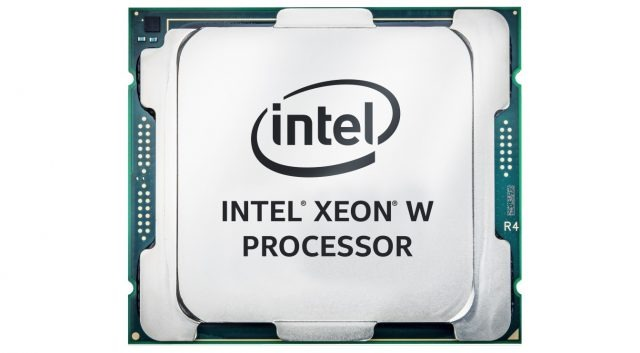
\includegraphics[width = 0.9\textwidth]{pic/process.jpg}
    \caption{Computer processor}
    \label{fig:fig7}
\end{figure}\\
We know that the a program or instruction will run / process fast depending on powerful processor. In~\cite{c.realme.comWebsite},Kotian, provided that in 2010 5.2 GHz was the top speed of processors by 2050 if engineers find a way to keep up with Moore's law and if processor speed actually develops every 24 months by 2050 we can get a chip capable of running at 5,452,595 gigahertz or nearly 5.5 petahertz.In 2050 the processor will be more powerful. So any task will be done using computer so fast that we can not imagine now.\\
I also think that in 2050 there will not use the keyboards that we use now. Instead a touch panel will be used for keyboard. This type of keyboard will be connected to computer via special data transfer medium.\\
The mouse as a pointer will not be used. Instead Human fingers will be used for mouse pointer.every thing where mouse is used there human fingers will be used.\\
I predict that futuristic computers/laptops might be invisible. We can use this pervasive computing as type of technology. This would incorporate our computers into anything's like vehicles, highways, clothing.  We wear today might have inbuilt computer elements coupled with networking technology. In 2050 the world around us will be a part of massive computing system.\\
I think in future medical sector will fully depend on computer and technology related devices. Different types of complex operations will be done by computers and robots, in present We can see it but rearly. Then every test and report will be done machines and prescription will be given as per diseases by computers. In future technology will reduce medical doctors and everything will be monitored by computers. Even a specific operation will be less cost in future.
I think that in 2050 computer and modern technology will be used in every small and big shopping malls. Even there will have robots for selling and attracting customers for coming to the malls. And transaction will totally be done electric money. All people use banking card for transactions. \\
I think in future every people will have a personal computer for their daily activities.
\subsection{Mobile phone in 2050}
Mobile phone is one of the important devices for our daily life. We can not move a step without mobile phone. Mobile is a device which is used for communicating with other.By using today's mobile phone, we can play video game, we can access internet with high band-with network, we can take high resolution picture instead using camera device.\\
\begin{figure}[h]
    \centering
    \begin{minipage}[b]{.49\textwidth}
    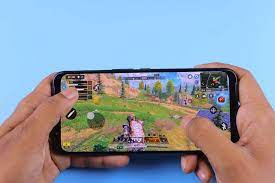
\includegraphics[width = 1\linewidth]{pic/gam.jpeg}
     \caption{Video gaming} 
     \label{fig:fig8}
    \end{minipage}
    %ggy
    \begin{minipage}[b]{.49\textwidth}
    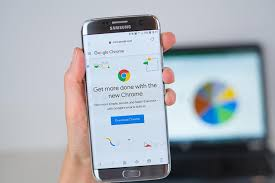
\includegraphics[width = 1\linewidth]{pic/brows.jpeg}
     \caption{Internet browsing} 
     \label{fig:fig9}
    \end{minipage} 
    %fddg
    \begin{minipage}[b]{.49\textwidth}
    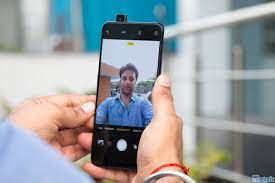
\includegraphics[width = 1\linewidth]{pic/camera.jpeg}
     \caption{Mobile camera} 
     \label{fig:fig10}
    \end{minipage}
\end{figure}\\
I think that in 2050 every features I have shown in figure~\ref{fig:fig8}, figure~\ref{fig:fig9} and figure~\ref{fig:fig10} will be much more updated. I think in 2050 mobile phone will take any one picture automatically when he or she will open camera and camera will detect faces. In future browsing using mobile phone will be more easier than the current period with high band-with. In 2050 Mobile phone will contain powerful processor and higher ram, then a gamer will be able to play video game it attractively.  \\
In~\cite{electronics.howstuffworks.comWebsite},Strickland, provided that in Based upon phone customer behavior, I imagine that the future phones will rely more on integrating our physical lives with our digital lives. They probably will not resemble the handsets we are used to now. They will be built into other devices and products. I will Imagine a pair of glasses that will display a digital overlay on top of my physical surroundings.\\
Since I am  talking 2050 here, there's even the possibility that research into brain-computer interfaces will have reached a point in which we will not need a physical screen or microphone at all. Electronics could be built into clothing or other accessories. Anyone would link the devices to an interface connected to your brain and direct applications and messages just through thought. It will be a technologically assisted form of telepathy.\\
I also think that the future mobile phone will attach with hand watch. It will be used as a hand watch as well as a mobile phone shown in figure~\ref{fig:fig11}.\\
\begin{figure}[h]
    \centering
    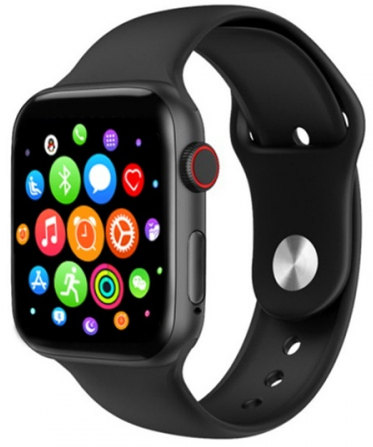
\includegraphics[width = 0.6\textwidth]{pic/handwatch.jpg}
    \caption{Hand watch smart phone}
    \label{fig:fig11}
\end{figure}\\
I think that in future by the welfare of technology it will be possible to control the satellites using powerful application.Mobile phone will also used in bio-medical sector. For example it will be able to detect internal diseases of human body using powerful camera and software. In future every mobile phone will be water-proof, so then there will not have the fear of damaging mobile phone when it will fall in water unconsciously by people.\\



